\documentclass{article}
\usepackage[utf8]{inputenc}
\usepackage{graphicx}
\usepackage{titling}
\usepackage{float}


\setlength{\parindent}{0pt}
% 1. Set professional margins (1 inch is standard)
\usepackage[margin=1in]{geometry}

% 2. Adjust the title height
\setlength{\droptitle}{-0.5in} 

\title{Labwork 2 - Linear Regression}
\author{Do Minh Quang - 2540095}
% \date{May 2026}

\begin{document}
\maketitle

\section{Dataset Overview}
The dataset is provided inside the labwork contains 2 numerical columns \textit{Area} and \textit{Price}.  We aim to find a linear relationship that shows how the price changes as the area increases.
\section{Linear Regression Implementation}
This labwork is for implementing linear regression algorithm from scratch using the function:
\[y = w_1 \times x + w_0\]

In order to determine the optimal weights $w_1$ and $w_2$, MSE is used as the loss function. The loss function for all the data points is:
\[J = \frac{1}{N} \sum^{N}_{i=1} L_i\]
where:
\begin{itemize}
    \item $N$ is the total number of data points
    \item $L_i$ is the single loss value of 1 data point. $L_i = \frac{1}{2} \times (\hat{y}_i - y_i)^2$
\end{itemize}

Then, this loss must be minimized using the Gradient Descent algorithm that we have done in the previous labwork.

\[w_0 = w_0 - lr * \frac{dL}{dw_0} ; w_1 = w_1 - lr * \frac{dL}{dw_1}\]

\begin{figure}[H]
    \centering
    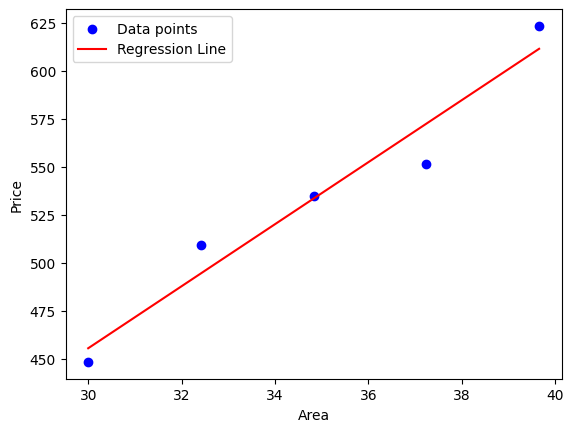
\includegraphics[width=0.8\linewidth]{Figure/lr.png}
    \caption{Linear Regression}
    \label{fig:lr}
\end{figure}

\end{document}